\tikzset{
    dots/.style={
        line width=4pt,
        line cap=round,
        dash pattern=on 0pt off 6pt
    }
}
\begin{tikzpicture}[scale=1.25]
\draw (0,4.25) rectangle (5,0);
%\node[anchor=south west] at (-0.9,-.2) {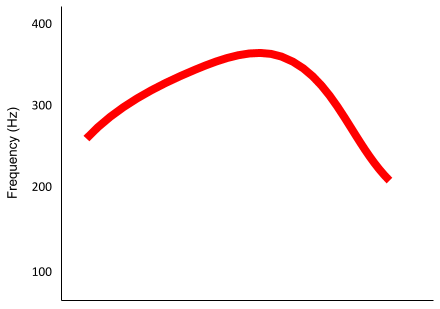
\includegraphics[scale=.4]{ranges-what-if1.png}};
\node[rotate=90] at (-0.75,2.2) {\relsize{-2}f0 (Hz)};
\begin{scope}[anchor=east, style={font=\relsize{-2}}]
	\node at (0,0) {0};
	\node at (0,1) {100};
	\node at (0,2) {200};
	\node at (0,3) {300};
	\node at (0,4) {400};
\end{scope}
\foreach \y in {2,...,4}
{
	\draw (0,\y) -- (-.1,\y);
}

\coordinate (pt1) at (0.4,2.5);
\coordinate (pt2) at (2.7,3.6);
\coordinate (pt3) at (3.3,3.5);
\coordinate (pt4) at (4.75,1.9);
\draw[dots, CB1] (pt1) .. controls (pt2) and (pt3) .. (pt4);
\end{tikzpicture}